\documentclass[twoside,openright,titlepage,fleqn,
	headinclude,11pt,a4paper,BCOR5mm,footinclude
	]{scrbook}
%--------------------------------------------------------------
        \newcommand{\myTitle}{Modelli statistici\xspace}
% use the right myDegree option
\newcommand{\myDegree}{Corso di Laurea Magistrale in Informatica\xspace}
%\newcommand{\myDegree}{
	%Corso di Laurea Specialistica in Scienze e Tecnologie 
	%dell'Informazione\xspace}
\newcommand{\myName}{Massimo Nocentini\xspace}
\newcommand{\myProf}{Giovanni Maria Marchetti\xspace}
\newcommand{\myOtherProf}{Nome Cognome\xspace}
\newcommand{\mySupervisor}{Nome Cognome\xspace}
\newcommand{\myFaculty}{
	Facolt\`a di Scienze Matematiche, Fisiche e Naturali\xspace}
\newcommand{\myDepartment}{
	Dipartimento di Sistemi e Informatica\xspace}
\newcommand{\myUni}{\protect{
	Universit\`a degli Studi di Firenze}\xspace}
\newcommand{\myLocation}{Firenze\xspace}
\newcommand{\myTime}{Anno Accademico 2012-2013\xspace}
\newcommand{\myVersion}{Version 0.1\xspace}

%--------------------------------------------------------------
\usepackage[latin1]{inputenc} 
\usepackage[T1]{fontenc} 
\usepackage[square,numbers]{natbib} 
\usepackage[fleqn]{amsmath}  
\usepackage[italian]{babel}
\usepackage{ae,aecompl}
\usepackage{graphicx}
\usepackage{latexsym}
\usepackage{amsmath, amsthm, amssymb}
\usepackage{rotating}
\usepackage{boxedminipage}
\usepackage{multicol}

%--------------------------------------------------------------
\usepackage{dia-classicthesis-ldpkg} 
%--------------------------------------------------------------
% Options for classicthesis.sty:
% tocaligned eulerchapternumbers drafting linedheaders 
% listsseparated subfig nochapters beramono eulermath parts 
% minionpro pdfspacing
\usepackage[eulerchapternumbers,subfig,beramono,eulermath,
	parts]{classicthesis}
%--------------------------------------------------------------
\newlength{\abcd} % for ab..z string length calculation
% how all the floats will be aligned
\newcommand{\myfloatalign}{\centering} 
\setlength{\extrarowheight}{3pt} % increase table row height
\captionsetup{format=hang,font=small}
%--------------------------------------------------------------
% Layout setting
%--------------------------------------------------------------
\usepackage{geometry}
\geometry{
	a4paper,
	ignoremp,
	bindingoffset = 1cm, 
	textwidth     = 13.5cm,
	textheight    = 21.5cm,
	lmargin       = 3.5cm, % left margin
	tmargin       = 4cm    % top margin 
}
%--------------------------------------------------------------
\usepackage{listings}
\usepackage{hyperref}
% My Theorem
\newtheorem{oss}{Observation}[section]
\newtheorem{exercise}{Exercise}[section]
\newtheorem{thm}{Theorem}[section]
\newtheorem{cor}[thm]{Corollary}

\newtheorem{lem}[thm]{Lemma}

\newcommand{\vect}[1]{\boldsymbol{#1}}

% questo comando e' relativo alle correzioni che puo
% apportare il prof se lo desidera.
\newcommand{\prof}[1]{\boldsymbol{#1}}

% instead of boldsymbol I can use the arrow above the letter with
%\newcommand{\vect}[1]{\vec{#1}}

% page settings
% \pagestyle{headings}
%--------------------------------------------------------------
\begin{document}
\frenchspacing
\raggedbottom
\pagenumbering{roman}
\pagestyle{plain}
%--------------------------------------------------------------
% Frontmatter
%--------------------------------------------------------------
%--------------------------------------------------------------
% titlepage.tex (use thesis.tex as main file)
%--------------------------------------------------------------
\begin{titlepage}
	\begin{center}
   	\large
      \hfill
      \vfill
      \begingroup
			\spacedallcaps{\myUni} \\ 
			\myFaculty \\
			\myDegree \\ 
			\vspace{0.5cm}
         
\includegraphics[scale=.065]{logo/unifi}\\
         \vspace{0.5cm}    
         %% -------put here the type of document---ie: Tesi di Laurea
         Elaborato d'Esame
      \endgroup 
      \vfill 
      \begingroup
      	\color{Maroon}\spacedallcaps{\myTitle} \\ \bigskip
      \endgroup
      \spacedlowsmallcaps{\myName}
      \vfill  
      Professore: \itshape{\myProf}
      \vfill  
      \myTime
      \vfill                      
	\end{center}        
\end{titlepage}   
%--------------------------------------------------------------
% back titlepage
%--------------------------------------------------------------
   \newpage
	\thispagestyle{empty}
	\hfill
	\vfill
	\noindent\myName: 
	\textit{\myTitle,} 
	\myDegree, \textcopyright\ \myTime
%--------------------------------------------------------------
% back titlepage end
%--------------------------------------------------------------
\pagestyle{scrheadings}
%--------------------------------------------------------------
% Mainmatter
%--------------------------------------------------------------
\pagenumbering{arabic}

% settings for the lstlisting environment
\lstset{
	language = R
	, numbers = left 
	, basicstyle=\sffamily%\footnotesize
%	, frame=single
	, tabsize=2
	, captionpos=b
	, breaklines=true
	, showspaces=false
	, showstringspaces=false
}

\tableofcontents

\newpage

\section*{Introduzione}
Queste note contengono tutto il mio materiale di studio per l'esame di
\emph{Modelli Statistici}.

\subsection*{Sintassi esercizi}
Per gli esercizi utilizziamo la sintassi \textbf{Exercise n[(m)]},
dove $n$ rappresenta la numerazione locale all'interno delle sezioni
di questo documento, $m$ rappresenta l'identificativo dell'esercizio
fissato nel documento \\
\href{http://www.ds.unifi.it/gmm/resources/capitoli.pdf}{
  http://www.ds.unifi.it/gmm/resources/capitoli.pdf}\\
Il reference $(m)$ non \`e sempre presente, come evidenziato dall'uso
delle parentesi quadre.


\newpage

\section*{Licenze}

Solo questa sezione dedicata alle licenze verr\`a scritta completamente in
inglese.

\subsection*{Text contents}
All the text content is distributed under:\\
\textbf{ This work is licensed under the Creative Commons Attribution,
  NonCommercial, ShareAlike 3.0 Unported License. To view a
  copy of this license, visit\\
  \href{http://creativecommons.org/licenses/by-nc-sa/3.0/}{http://creativecommons.org/licenses/by-nc-sa/3.0/}\\
  or send a letter to Creative Commons, 444 Castro Street, Suite 900,
  Mountain View, California, 94041, USA.}

\begin{center}

\includegraphics{cc-icons-eps/by}

\includegraphics{cc-icons-eps/cc}

\includegraphics{cc-icons-eps/nc}

\includegraphics{cc-icons-eps/sa}
\end{center}

\subsection*{Sources}
All sources are distributed under, where the word ``Software'' is
referred to all of the sources that are present in this work: \\
\textbf{
  Copyright (c) 2011 Massimo Nocentini\\
  Permission is hereby granted, free of charge, to any person
  obtaining a copy of this software and associated documentation files
  (the "Software"), to deal in the Software without restriction,
  including without limitation the rights to use, copy, modify, merge,
  publish, distribute, sublicense, and/or sell copies of the Software,
  and to permit persons to whom the Software is furnished
  to do so, subject to the following conditions:\\
  The above copyright notice and this permission notice shall be
  included in all
  copies or substantial portions of the Software.\\
  THE SOFTWARE IS PROVIDED "AS IS", WITHOUT WARRANTY OF ANY KIND,
  EXPRESS OR IMPLIED, INCLUDING BUT NOT LIMITED TO THE WARRANTIES OF
  MERCHANTABILITY, FITNESS FOR A PARTICULAR PURPOSE AND
  NONINFRINGEMENT. IN NO EVENT SHALL THE AUTHORS OR COPYRIGHT HOLDERS
  BE LIABLE FOR ANY CLAIM, DAMAGES OR OTHER LIABILITY, WHETHER IN AN
  ACTION OF CONTRACT, TORT OR OTHERWISE, ARISING FROM, OUT OF OR IN
  CONNECTION WITH THE SOFTWARE OR THE USE OR OTHER DEALINGS IN THE
  SOFTWARE.  }


\chapter{Stima, verifica d'ipotesi e distribuzioni campionarie}

\begin{exercise}{\emph{(2.6 nel testo)}}
  Considerate il modello in cui $Y_1,\ldots, Y_n$ sono indipendenti e
  identicamente distribuite come una uniforme $Y \sim U(0, \theta)$,
  dove $\theta$ \`e il valore massimo che pu\`o assumere $Y$.
  Determinate per simulazione la distribuzione campionaria di $T = 2Y$
  considerando $\theta = 100, n = 20$. Mostrate con un istogramma che
  la distribuzione dello stimatore \`e approssimabile da una
  normale. Qual \`e la varianza di $T$? Usate questa varianza per
  sovrapporre all'istogramma la curva normale che lo approssima
  (ricordate di disegnare l'istogramma in R con l'opzione freq =
  FALSE).
\end{exercise}
Questo il codice che implementa l'esercizio:
\lstinputlisting{r-sources/exercises/chapter-two/two-six.R}
Vediamo qualche risultato inserendo in R:
\begin{lstlisting}
  > twosix()
  $estimatorVector
    [1]  95.96794 105.40497 110.64482  89.14495 107.99978 116.03221
    94.73158 ...
  
  $empiricalMean
  [1] 100.2173

  $empiricalVar
  [1] 168.8848

  $empiricalVarComputedByHand
  [1] 168.8848

  $sd
  [1] 12.99557
\end{lstlisting}
L'esecuzione della funzione produce la \autoref{fig:two-six}, dove la
curva in blu rappresenta la densit\`a inferita usando gli algoritmi
disponibili in R dello stimatore $2\bar{Y}$, mentre la curva in rosso
rappresenta il modello esatto usando come parametri i valori stimati
dalla media e dalla varianza campionaria (riportate nel precedente
output come \texttt{empiricalMean} e \texttt{empiricalVar}).
\begin{figure}[htb]
\centering
\includegraphics[height=13cm,width=13cm]{r-sources/exercises/chapter-two/two-six.ps}
\caption{Istogramma esercizio 2.6 del testo}
\label{fig:two-six}
\end{figure}

\begin{exercise}{\emph{(2.7 nel testo)}}
  Una azienda chimica ha prodotto un additivo per la benzina che
  dovrebbe migliorare il consumo oltre le 25 miglia per
  gallone. Viene fatto un esperimento con 30 auto uguali su un
  percorso standard e si ottiene un consumo medio di 26.3 mpg con una
  deviazione standard campionaria di 2.4 mpg. Trovare un intervallo di
  confidenza al $95\%$ per il consumo medio supponendo il modello normale.
\end{exercise}
Questo il codice che implementa l'esercizio:
\lstinputlisting{r-sources/exercises/chapter-two/two-seven.R} Nel
campionamento ripetuto l'intervallo di confidenza riportato sotto
conterr\`a il vero valore del parametro (consumo medio) con una
probabilit\`a di copertura del 95\%.
\begin{lstlisting}
  > twoSeven()
  $tOss
  [1] 2.966831

  $confidenceInterval
  [1] 25.40383 27.19617

  $pValue
  [1] 0.002986329
\end{lstlisting}
Inoltre abbiamo condotto un test di significativit\`a per verificare
se l'additivo \`e efficacie o meno. Per questo mettiamo come ipotesi
nulla $H_0:$``con un gallone si fanno meno di 25 miglia'' (che
speriamo di rifiutare) contrapposta a $H_1:$``con un gallone si fanno
almeno 25 miglia''. Dall'esecuzione del nostro codice otteniamo un
\emph{p-value} uguale a 0.002, pertanto il test risulta significativo,
rifiutiamo $H_0$, l'additivo \`e efficacie. \`E da notare che in
questo caso non \`e stato possibile utilizzare gli algoritmi messi a
disposizione in R per il test di significativit\`a in quanto non si ha
il campione visibile (nel prossimo esercizio invece sar\`a possibile
effettuare il test sia in modo automatico che manuale).

\begin{exercise}{\emph{(2.8 nel testo)}}
  Un misuratore del tasso di alcool nel sangue viene verificato su un
  campione di prova in cui la misura dovrebbe essere 12\%. Trovare una
  stima della media e il suo errore standard. Trovare un intervallo di
  confidenza a livello del 95\% per la media col modello normale. Fare
  un test dell'ipotesi che il misuratore sia correttamente calibrato
  cio\`e che $\mu = 12$ contro l'alternativa che $\mu \not = 12$.
\end{exercise}
Questo il codice che implementa l'esercizio:
\lstinputlisting{r-sources/exercises/chapter-two/two-eight.R}
Vediamo qualche risultato inserendo in R:
\begin{lstlisting}
  > twoEight()
  $automaticTest

  One Sample t-test

  data:  alcoholValues 
  t = 12.7718, df = 29, p-value = 1.964e-13
  alternative hypothesis: true mean is not equal to 12 
  95 percent confidence interval:
  12.63550 12.87784 
  sample estimates:
  mean of x 
  12.75667 


  $tOss
  [1] 12.77184

  $confidenceInterval
  [1] 12.63550 12.87784

  $pValue
  [1] 1.963566e-13
\end{lstlisting}
Il test risulta altamente significativo, l'ipotesi nulla $\mu=12$
viene rifiutata pertanto il misuratore non \`e correttamente
calibrato.


\begin{exercise}{(2.10 nel testo)}
  Si studia un campione di 100 individui e si considera il numero di
  vegetariani.  Si sono osservati $r = 2$ vegetariani su $n = 100$
  prove (supposte Bernoulli indipendenti e identiche). Trovare
  l'intervallo di confidenza asintotico al 95\% per la proporzione di
  vegetariani nella popolazione. Notare che l'intervallo ha il limite
  inferiore negativo. Calcolare anche l'intervallo di Agresti e Coull.
\end{exercise}
Questo il codice che implementa l'esercizio:
\lstinputlisting{r-sources/exercises/chapter-two/two-ten.R} Osserviamo
dall'output riportato sotto che l'intervallo di confidenza calcolato
con il metodo asintotico ha l'intervallo inferiore negativo, mentre
non \`e cos\`i per quello calcolato con la correzione Agresti-Coull.
\begin{lstlisting}
  > twoTen()
  $asymptotic
  [1] -0.007439496  0.047439496

  $AgrestiCoull
  [1] 0.001501869 0.075421208
\end{lstlisting}


\chapter{Modelli per il confronto tra gruppi}
\begin{exercise}{\emph{(3.1 nel testo)}}
  Per verificare quanto tempo impiega il poliestere a deteriorarsi in
  una discarica, un ricercatore ha preso 10 strisce di poliestere e le
  ha interrate. Cinque strisce scelte a caso sono state estratte dopo
  due settimane e le restanti dopo 3 mesi. Su ogni striscia \`e stata
  misurata la forza di rottura in libbre. Sono state ottenute le
  statistiche seguenti.
  \begin{table}[h]              % 'h' for 'here' position
    \centering
    \begin{tabular}{|c|c|c|c|}
      \hline
      Gruppo & n & media & sd \\\hline
      2 settimane & 5 & 123.8 & 4.6 \\
      3 mesi & 5 & 116.4 & 16.09 \\ \hline
    \end{tabular}
  \end{table}
  Costruire un intervallo di confidenza al 95\% per la differenza
  delle medie assumendo la normalit\`a e l'omoschedasticit\`a.
  Sottoporre a test l'ipotesi di uguaglianza delle medie.
\end{exercise}
Questo il codice che implementa l'esercizio:
\lstinputlisting{r-sources/exercises/chapter-three/three-one.R} Nel
campionamento ripetuto l'intervallo di confidenza riportato sotto
conterr\`a il vero valore del parametro (differenza delle medie) con una
probabilit\`a di copertura del 95\%.
\begin{lstlisting}
  > threeOne()
  $tOss
  [1] 0.9887817

  $meansDifference
  [1] 7.4

  $confidenceInterval
  [1] -9.858037 24.658037

  $pValue
  [1] 0.3517289
\end{lstlisting}
La differenza delle medie non \`e significativa pertanto si mantiene
l'ipotesi che le due medie siano uguali e che il trattamento non ha
avuto effetto.

\begin{exercise}{\emph{(3.3) nel testo}}
  I dati seguenti rappresentano i pesi di 20 uomini partecipanti a un
  programma di perdita di peso, prima e dopo il programma.  Vogliamo
  sapere se in media il programma ha avuto effetto. Fare un test
  oppor- tuno esplicitando le assunzioni.
\end{exercise}
Non possiamo procedere allo studio della differenza delle medie
campionarie dei due gruppi: i due campioni $Y=(Y_1, \ldots, Y_{20})$ e
$Y' = (Y'_1, \ldots, Y'_{20})$ non sono indipendenti, in quanto $(Y_i,
Y'_i)$ sono il peso della persona $i$-esima e quindi il modello non
\`e applicabile direttamente.

Per questo motivo costruiamo il campione $(Y_1-Y'_1, \ldots,
Y_{20}-Y'_{20})$: questo nuovo oggetto viene costruito a partire dai
campioni originari, tra loro indipendenti ma non identicamente
distribuiti, piu' formalmente $(Y_1, \ldots, Y_{20})$ si suppone
distribuito come $N(\mu_1, \sigma^2)$, mentre $(Y'_1, \ldots,
Y'_{20})$ si suppone distribuito come $N(\mu_2, \sigma^2)$.

Per tanto il campione differenza ha distribuzione campionaria data da
$N(\bar{Y} - \bar{Y'}, var(Y) + var(Y') -2cov(Y, Y'))$, chiariamo la
varianza:
\begin{displaymath}
  \begin{split}
    var(Y - Y') &= var(Y + (-Y')) = var(Y) + (-1)^2var(Y') +
    2cov(Y,-Y') \\
    &= var(Y) + var(Y') + 2E\left((Y-E(Y))(-Y'-E(-Y')) \right) = \\
    &= var(Y) + var(Y') + 2E\left((Y-E(Y))(-Y'+E(Y')) \right) = \\
    &= var(Y) + var(Y') - 2E\left((Y-E(Y))(Y'-E(Y')) \right) = \\
    &= var(Y) + var(Y') - 2cov(Y,Y')
  \end{split}
\end{displaymath}
Questo il codice che implementa l'esercizio:
\lstinputlisting{r-sources/exercises/chapter-three/three-three.R}
Abbiamo fissato l'ipotesi nulla $H_0$ che la media del nuovo campione
(ovvero delle differenze tra prima e dopo la dieta) sia uguale a 0 ad
un livello del 95\%, con una ipotesi alternativa unilaterale (in
quanto speriamo di avere una perdita di peso):
\begin{lstlisting}
> threeThree()
$sample
[1]  3.8 -5.5  8.9  0.0  8.0  5.2  7.7  7.5  5.0  0.8  0.0  2.6  9.0 -3.6  0.1
[16]  0.5  2.0  0.0  0.9  0.0

$automaticTest

One Sample t-test

data:  sample 
t = 2.8734, df = 19, p-value = 0.004865
alternative hypothesis: true mean is greater than 0 
95 percent confidence interval:
1.053314      Inf 
sample estimates:
mean of x 
2.645 


$empiricalMean
[1] 2.645

$tOss
[1] 2.873404

$confidenceInterval
[1] 0.718348 4.571652

$pValue
[1] 0.004865231
\end{lstlisting}
La differenza \`e altamente significativa pertanto si rifiuta $H_0$ e
il trattamento ha avuto effetto.



\end{document} 
